
\paragraph{} This chapter will cover a number of topics essential to understanding the rationale and implementation of the design as discussed in §~\ref{sec:design}. These include; Intel SGX, a brief overview of modern \textit{libOSes}, an introduction to \textit{Information Flow Control} (\textit{IFC}), and a overview of key aspects of the Linux kernel relevant to the architecture of the prototype.

\section{Intel SGX}

\paragraph{} Intel's Software Guard Extensions, SGX, was first announced and detailed in a handful of whitepaper documents published in 2013. [X,Y,Z] It described a novel approach, creating in-CPU containers with their own protected memory pools. These regions, called \textit{enclaves}, cannot be read from or written due to fundamental protection mechanisms provided by the x86 architecture. \textit{Enclaves} provide both integrity and secrecy to the operation running inside of it, even in the prescence of a malicious host.

\paragraph{Motivation} At a high level SGX aims to achieve security for sensitive application by shielding them, and the resources it uses, against tampering and to provide a guarantee to end users about the an enclaves integrity; this is achieved using measurement and attestation. A driving use case is in a cloud computing context, where users are forced to trust a foreign party with both their data and business logic. By distributing encrypted, yet executable, containers targetting a single, unique SGX CPU, users can be assured that their information is safe, regardless of any virutalisation that may be taking place. Only the provisioned CPU is able to decrypt and execute the enclave, strictly in accordance with the restrictions of the SGX platform.

\subsection{Security Characteristics}

\begin{figure}[]
    \centering
    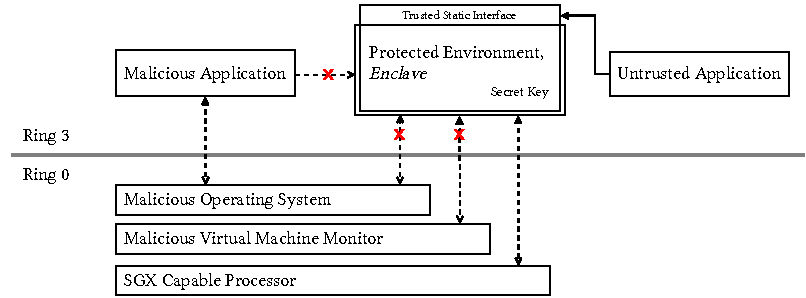
\includegraphics[width=0.9\linewidth]{figures/SGX-architecture.pdf}
    \caption{Abstract overview of an SGX enclave's protections}
    \label{fig:sgx-basic}
\end{figure}

\paragraph{} At its heart SGX is designed to be \textit{trustworthy}; this is achieved in a number of ways, including robust enclaving provisioning, sealing and attestation. Intel enumerates SGX's protections as follows;

\begin{itemize}
    \item Memory security against observation and modification from outside the enclave; this is achieved using an in-die \textit{Memory Encryption Engine} (\textit{MEE}), with a secret that rotates on every boot. This protection notably works against a host hypervisor, other enclaves, and anything running in supervisor mode.
    \item Attestation of an enclave to a challenger through the use of a permanent hardware security key for asymmetric encryption.
    \item Proxied software calls to prepare and transfer control in and out of an enclave. Arguments are securely marshalled according to a static enclave definition.
    \item SGX does not defend against reverse engineering or sidechannel attacks: [X,Y] this is the responsibility of the developer to mitigate.
    \item Debugging support is only provided via a specialised tool and only when an enclave is compiled with debugging enabled.
\end{itemize}

\subsection{Architecture and Implementation}

\begin{figure}[]
    \centering
    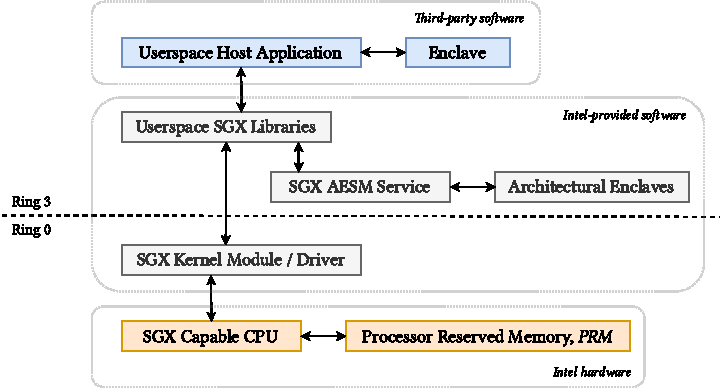
\includegraphics[width=0.9\linewidth]{figures/SGX-AdvArchitecture.pdf}
    \caption{A high-level overview of the SGX hardware and software architecture.}
    \label{fig:sgx-advarch}
\end{figure}

\paragraph{} The SGX platform comprises a number of interlocking parts, as shown in Figure~\ref{fig:sgx-advarch}. Working from the hardware up, at the heart of the platform is the extended x86 instruction set and memory protection provided by an SGX-capable CPU. 

\paragraph{Hardware} Enclaves' data and code is stored securely in \textit{Processor Reserved Memory}, \textit{PRM}; this is a set of pages in system memory that are presided over by the \textit{MEE}. DMA\footnote{Direct Memory Access} to \textit{PRM} is always rejected. \textit{PRM} consists of two datastructures; the \textit{Enclave Page Cache Map} (\textit{EPCM}) and the \textit{Enclave Page Cache} (\textit{EPC}). An individual enclave is defined by an \textit{SGX Enclave Control Structure}, \textit{SECS}; this is generated when an enclave is created and stored in a dedicated entry in the \textit{EPC}. An enclave's \textit{SECS} contains important information such as its (system) global identifier, its measurement hash and the amount of memory it is using. Access control information is stored in the \textit{EPCM} alongside page validity flags, the owning enclave identifier and the page's type; this is not accessible from software. An attempt to resolve a page in \textit{PRM} is successful only if the CPU is executing in enclave mode and its \textit{EPCM} entry states it belongs the currently executing enclave --- if this is not the case the lookup returns an unused page from generci system memory.

\paragraph{} The host OS or hypervisor manages the \textit{EPC} just as it does with normal system memory, swapping pages in and out according to its own policy, but must do so using SGX specific instructions. The \textit{MEE} is responsible for ensuring the integirty and confidentiality of this process, encrypting and decrypting pages as they cross the \textit{PRM} boundary. Data is verified with the use of an integrity tree, and encryption keys are generated at boot-time. Importantly the SGX archicture relies on the host OS to be SGX-aware, empowering userspace applications to function without the priviliedge; this is provided by the SGX driver, \textit{isgx}.

\paragraph{} Kernel module, driver. SDK.

\subsection{Enclave Lifecycle}

\subsection{Attestation}

\subsection{Provisioning and Sealing}

\section{Modern \textit{libOSes}}

\section{Information Flow Control}

\section{Aspects of the \textit{Linux} Kernel}